\documentclass{book}

%%%%

%% Theorem-like environments

%% http://www.maths.tcd.ie/~dwilkins/LaTeXPrimer/Theorems.html
%% https://www.sharelatex.com/learn/Theorems_and_proofs
%% http://tex.stackexchange.com/a/46262
\newtheorem{theorem}{Theorem}[section]
\newtheorem{lemma}[theorem]{Lemma}
\newtheorem{proposition}[theorem]{Proposition}
\newtheorem{corollary}{Corollary}[theorem]
\newtheorem{remark}{Remark}[section]
\newcommand{\remarkautorefname}{Remark}

%% Adapted from https://tex.stackexchange.com/q/45817
\theoremstyle{definition}
\newtheorem{definition}{Definition}[section]
\newtheorem{axiom}{Axiom}[section]
\newtheorem{conjecture}{Conjecture}[section]
\newtheorem{example}{Example}[section]

%%%%

\newcommand{\ch}{{c.}\:}             % chapter in bib citations
\newcommand{\s}{{s.}\:}              % section in bib citations
\newcommand{\citeplace}[1]{{#1}\:}   % ``any'' in bib citations  e.g. \cite[\citeplace{handout} 2]{Webber_notes}

\newcommand{\term}[1]{\emph{#1}}
\newcommand{\idop}{\mathbbm{1}}           % Identity operator
\newcommand{\hilb}[1]{\mathcal{#1}}       % Hilbert space
\newcommand{\setof}[1]{\left\{#1\right\}}
\newcommand{\ox}{\otimes}
\newcommand{\transpose}{\top}

%% Allows better formatting than \underset
%% https://tex.stackexchange.com/a/130553
\DeclareMathOperator*{\repr}{\,\equiv\,}      % represented in a basis, or "has components..."

\renewcommand{\op}{\hat}                  % overwriting physics \op = \ketbra
%\renewcommand{\op}{}                      % overwriting physics \op = \ketbra
\newcommand{\eqbydef}{\coloneqq}
%\newcommand{\eqbydef}{\triangleq}
\newcommand{\superop}{\mathcal}

\newcommand{\dket}[1]{\left.\left| #1 \right\rangle\right\rangle}
\newcommand{\Dket}[1]{\left.\left| #1 \right\rangle\!\right\rangle}
\newcommand{\dbra}[1]{\left\langle\left\langle #1 \right|\right.}
\newcommand{\Dbra}[1]{\left\langle\!\left\langle #1 \right|\right.}
\newcommand{\dbraket}[2]{\left\langle\left\langle #1 \middle| #2 \right\rangle\right.\!}
\newcommand{\bradket}[2]{\!\left.\left\langle #1 \middle| #2 \right\rangle\right\rangle}
\newcommand{\braDket}[2]{\!\left.\left\langle #1 \middle| #2 \right\rangle\!\right\rangle}
\newcommand{\dbradket}[2]{\left\langle\left\langle #1 \middle| #2 \right\rangle\right\rangle}
\newcommand{\dketdbra}[2]{\dket{#1}\dbra{#2}}

%% smaller than \quad but still quite larger than \;
\newcommand{\kuad}[0]{\:\:\,}

\newcommand{\pwspace}{\hilb{H}_T \ox \hilb{H}_S}

\NewEnviron{eqsplit}{\begin{equation}\begin{split}\BODY\end{split}\end{equation}}
\NewEnviron{eqsplit*}{\begin{equation*}\begin{split}\BODY\end{split}\end{equation*}}

% Imaginary unit (not used much this way here though)
% https://tex.stackexchange.com/a/303698
\newcommand{\iu}{\mathrm{i}\mkern1mu}
\newcommand{\E}{\mathrm{e}}

% Functions
% Heaviside function
\newcommand{\Hvsd}[1]{\Theta\left(#1\right)}

%\newcommand{\nullvector}{\underline{0}}
\newcommand{\nullvector}{0}


\author{Guido De Rosa \\ \small\tt{gderosa@umail.ucc.ie}}
\title{Time as a quantum observable: from Pauli objection to Page and Wootters model --- improvements and applications}

\begin{document}

\maketitle

\tableofcontents

\chapter*{Abstract}
A proof is detailed of the (in)famous Pauli's ``theorem''~\cite{PauliFootnote}
on the impossibility of a time observable in quantum mechanics. Some possible
approaches towards overcoming Pauli's objections are reviewd and expanded as well.

\chapter{Pauli's objection}
% sections
\section{Introduction}

In a footnote in~\cite{PauliFootnote}, W. Pauli excluded the possibility
of a self-adjoint operator representing time as a quantum observable.
However, he did not provide an explicit proof.
Here a proof is given, based on~\cite{Galapon2002}, but expanded in more detail.
\section{Proof of Pauli's formal argument}\label{proof}

Let's assume that there exists a self-adjoint time operator, $T$, canonically conjugate
to the Hamiltonian $H$, i.e.

\begin{equation}
\label{THcommutator}
[T, H] = i\hbar
\end{equation}
Since T is self-adjoint, then for all
$\beta\in\mathbb{R}$, $U_{\beta} = \exp(- i \beta T / \hbar)$
is unitary. A formal
expansion of the exponential yields the commutator

\begin{equation}
[U_{\beta}, H]  =
\left[
    \sum_{k=0}^{\infty} \frac{1}{k!} \left(- \frac{i\beta T}{\hbar} \right)^k, H
\right]         =
\sum_{k=0}^{\infty} \frac{1}{k!} \left(- \frac{i\beta}{\hbar} \right)^k [T^k, H]
\end{equation}.

As the commutator $[T, H]$ itself commutes with its operator $T$,
the following identity holds (See Lemma \ref{CommProp}):

$$
[T^k, H] = kT^{k-1}[T, H]
$$
hence:

\begin{multline}
[U_{\beta}, H]  =
\sum_{k=0}^{\infty} \frac{1}{k!} \left(- \frac{i\beta}{\hbar} \right)^k kT^{k-1}[T, H] \\ =
\beta\sum_{k=1}^{\infty} \frac{1}{(k-1)!} \left(- \frac{i\beta}{\hbar} \right)^{k-1} T^{k-1} =
\beta\sum_{\kappa=0}^{\infty} \frac{1}{\kappa!} \left(- \frac{i\beta T}{\hbar} \right)^{\kappa}  =
\beta U_{\beta}
\end{multline}
where the term for $k=0$ in the first sum clearly vanishes, hence we can start the sum from
$k=1$ then set $\kappa=k-1$.

Now, given an eigenvector $\varphi_{E}$ so that $H\varphi_{E}=E\varphi_{E}$, there has:

$$
HU_{\beta}\varphi_{E} = (U_{\beta}H - [U_{\beta}, H])\varphi_{E} =
EU_{\beta}\varphi_{E} - \beta U_{\beta}\varphi_{E} = (E-\beta)U_{\beta}\varphi_{E}
$$
showing that $U_{\beta}\varphi_{E}$ is another eigenvector of $H$ with eigenvalue
$E-\beta$. But $\beta$ is an arbitrary real number and $H$ a \emph{generic} Hamiltonian,
hence the spectrum of a generic Hamiltonian $H$ should
be the whole real line, which contradicts the discrete and semi-bounded energy spectrum
in fact found in most physical systems.

\chapter{Approaches}
% section
\section{Approaches}

They are

\begin{itemize}
\item early attempts reviewed in \cite{TQM1, TQM2}, Aharonov-Bohm, Kijowski etc.
\item detector model \cite{TQM1, TQM2}
\item
    time $\otimes$ position Hilbert space or ``second'' Schr\"odinger equation (Prvanovic)
\item time and entanglement (Page and Wootters model, Leggett-Garg inequality as \emph{time} version of Bell inequalities, experiments by Moreva, Genovese et al.)
\item approachs where not only spacetime but causality itself is not fundamental (indefinite causal order: Oreshkov, Brukner et al)
\item event-based approaches: 
    \begin{itemize}
        \item ``event'' wavefunction square integrable in 4D (how does it relate rigourously to detector model?)
        \item event-enhanced quantum theory (EEQT, Ruschhaupt et al.)
        \item 
    \end{itemize}
\end{itemize}

\chapter{Critical review of Page and Wootters mechanism and proposed improvements}
\chaptermark{Critical review of Page and Wootters \dots}
\section{Introduction}

The Page and Wootters model is based on
an additional Hilbert space $\mathcal{H}_T$,
where time is an observable
represented by a self-adjoint operator
whose properties are similar to the ones of position
in ordinary quantum mechanics
\parencite{Lloyd:Time, Maccone:Pauli}.

In this language, the ordinary Hilbert space can be labeled $\mathcal{H}_S$;
and we consider the product space $\mathcal{H}_T \otimes \mathcal{H}_S$ as
the space in which both time and position are observables, and they act as
$\hat{t} \otimes \idop_S$ and $\idop_T \otimes \hat{x}$
respectively.

\begin{remark}
  In a more ``relativistic friendly'' notation, we may set
  $\hat{x_0} = c\hat{t}$ and consider
  $\hat{x_0} \otimes \idop_S$ and $\idop_T \otimes \hat{x_1}$,
  and so on. An interesting development may be expressing
  Lorentz transformations as unitary transformations in
  $\mathcal{H}_T \otimes \mathcal{H}_S$.
\end{remark}

The Page and Wootters mechanism is rooted in the ``problem of time''
in quantum cosmology.
In principle, an approriate system (a ``clock'') can be identified in such a way
to be described in $\mathcal{H}_T$, while $\mathcal{H}_S$ describes
the quantum states of \emph{the rest of the universe} \parencite{Marletto:Evolution}.

As explained in \cite{Lloyd:Time, Maccone:Pauli}, the overall Hamiltonian,
encompassing both position and time as observables, is given by
\begin{equation}
  \hat{\mathbb{J}} = \hbar\hat{\Omega}\ox\idop_S + \idop_T\ox\hat{H}_S \,\text{,}
\end{equation}
while the \term{Wheeler-DeWitt equation} holds:
\begin{equation}
  \hat{\mathbb{J}}\dket{\Psi} = 0 \,\text{,}
\end{equation}
describing a \emph{static} universe, where evolution is only
in terms of relations between parts of a multipartite system
(a ``clock'' and ``the rest'').



\section{Theoretical developments following Moreva et al. experiment}

And an experiment: \cite{Moreva:synthetic,Moreva:illustration}.
Some theoretical implications of the experiment are reviewed in
\cite{LeggettGarg+PageWootters}.

And a NEW experiment! \parencite{Moreva_position}.


\iftodo

\section{Prvanovic and P\&W}
In \cite{Prvanovic}, essentially the clock observable is the Hamiltonian.
The two example clocks are an harmonic oscillator and a free particle.
The harmonic oscillator features discrete time. Generally a time which is
{bounded from below}
is consistent with the Big Bang...

Prvanovic uses ``relativisitc'' constants...

Ciao.

\section{Analyze latest Moreva experiment with previous ones}

Let's consider a photon, as a two level system with its two linear polarization
sates $\ket{H}, \ket{V}$;
and the Hamiltonian
\begin{equation}
  \mathcal{H}=i\hbar\omega\qty(\ket{H}\ket{V}-\ket{V}\ket{H})\,\text{.}
\end{equation}
There has:
\[
  \mathcal{H}^n \ket{H, V} = \begin{cases}
      \hbar^n\omega^n\ket{H, V} &\text{for n even} \\
    -i\hbar^n\omega^n\ket{V, H} &\text{for n odd}
  \end{cases}
\]

\url{http://physweb.bgu.ac.il/COURSES/PHYSICS3_physics/CLASS_ymeir/polarization.pdf}

\section{Entanglement and decoherence (Arrow of time)}
See also \cite{EntanglementVsDecoherence}.

Decoherence is an irreversible process, it also happens in measurement.

According to Marletto and Vedral, arrow of time is increase in Entanglement
between the clock and the rest.

So, there seems to be a contradiction: is entanglement ``decreasing''
(i.e. destroyed by decoherence) with time
or increasing?

We can avoid the contradiction saying that
entanglement between two finite systems is
destroyed while the entanglement of each of them with the universe
is increasing.

\fi

\iftodo
\section{TODOs}

TODO: \cite{RealisticClocks}.

\cite{HarmonicClocks} concludes ``Classical clock can be described by an Hamiltonian linear in momentum''\dots
like in relativity?

Extra: \cite{TimeAnyons}.

TODO: use the harmonic oscillator in \cite{HarmonicClocks}
as a PaW clock for the same packet that is measured in
Ruschhaupt's detector model.
Therein, fading wave function: is minus derivative an event?
L4 normalized?

Other systems of interest: decays. Prvanovic new.

TQM Book: time of residence: applicable to qubits, therefore Moreva experiment.

https://arxiv.org/abs/1708.04302 majorization, thermo.

\fi


\section{In relation to Leggett-Garg inequalities (TODO: move to another file)}
Ref \cite{LeggettGarg+PageWootters}.

But also Lloyd: \url{https://arxiv.org/abs/1608.05672},
\emph{Decoherent histories approach to the cosmological measure problem}.
Lindbladt, Markov, Open Systems.

Halliwell, \url{https://arxiv.org/abs/1604.01659}. Ancilla, decay (spontaneous emission?).

A phylosophical object to decoherent histories / Everett (Everett mentioned in Marletto/ref)
is at
\url{https://arxiv.org/abs/1603.04845}.



\chapter{When Time Crystals come into play}
% sections
\section{Intro}

References: \parencite{crystal2,crystal3,crystal2012}.

Maybe to be removed, if there is enuogh work in other chapters.


\chapter{Thermal time hypothesis}
% sections
\section{Connes and Rovelli}

Reference \parencite{ConnesRovelliThermo}.

\section{More}

Relate with John Goold's works? The ancilla as a clock? --- Topical Review

Markovianity, histories.

Lloyd on arXiv: from clock to cloners; erasing; scrambling (as in Goold).

Lloyd on decoherent histories (Gellman, Hartle?).

Dechoerence / irreversibility / measurement.

Vedral / Lloyd. Discord.

Measuring entanglement: Quantification of Concurrence via Weak Measurement: 1611.00149.

Marletto/Vedral on Arrow of time. Arrow of time as increasing entanglement.

Arrow of time: 

\url{https://www.wired.com/2014/04/quantum-theory-flow-time/}

\url{https://en.wikipedia.org/wiki/Loschmidt%27s_paradox}

\url{https://www.quantamagazine.org/20160119-time-entanglement/}

\section{Misc}

\url{https://arxiv.org/pdf/1702.07706.pdf} \textit{The second law of thermodynamics at the microscopic scale}
Thibaut Josset,
Aix Marseille Univ. (David).

Maxwell's demon: https://arxiv.org/pdf/1702.05161.pdf

\chapter{Extras}
% sections
\section{An intro chap on motivation and experiments?}
\begin{itemize}
  \item Time crystals?
  \item Time-resolved diffraction patters, temporal double slit experiment + Muga theory \url{https://arxiv.org/pdf/0812.3034.pdfß}
\end{itemize}

%\clearpage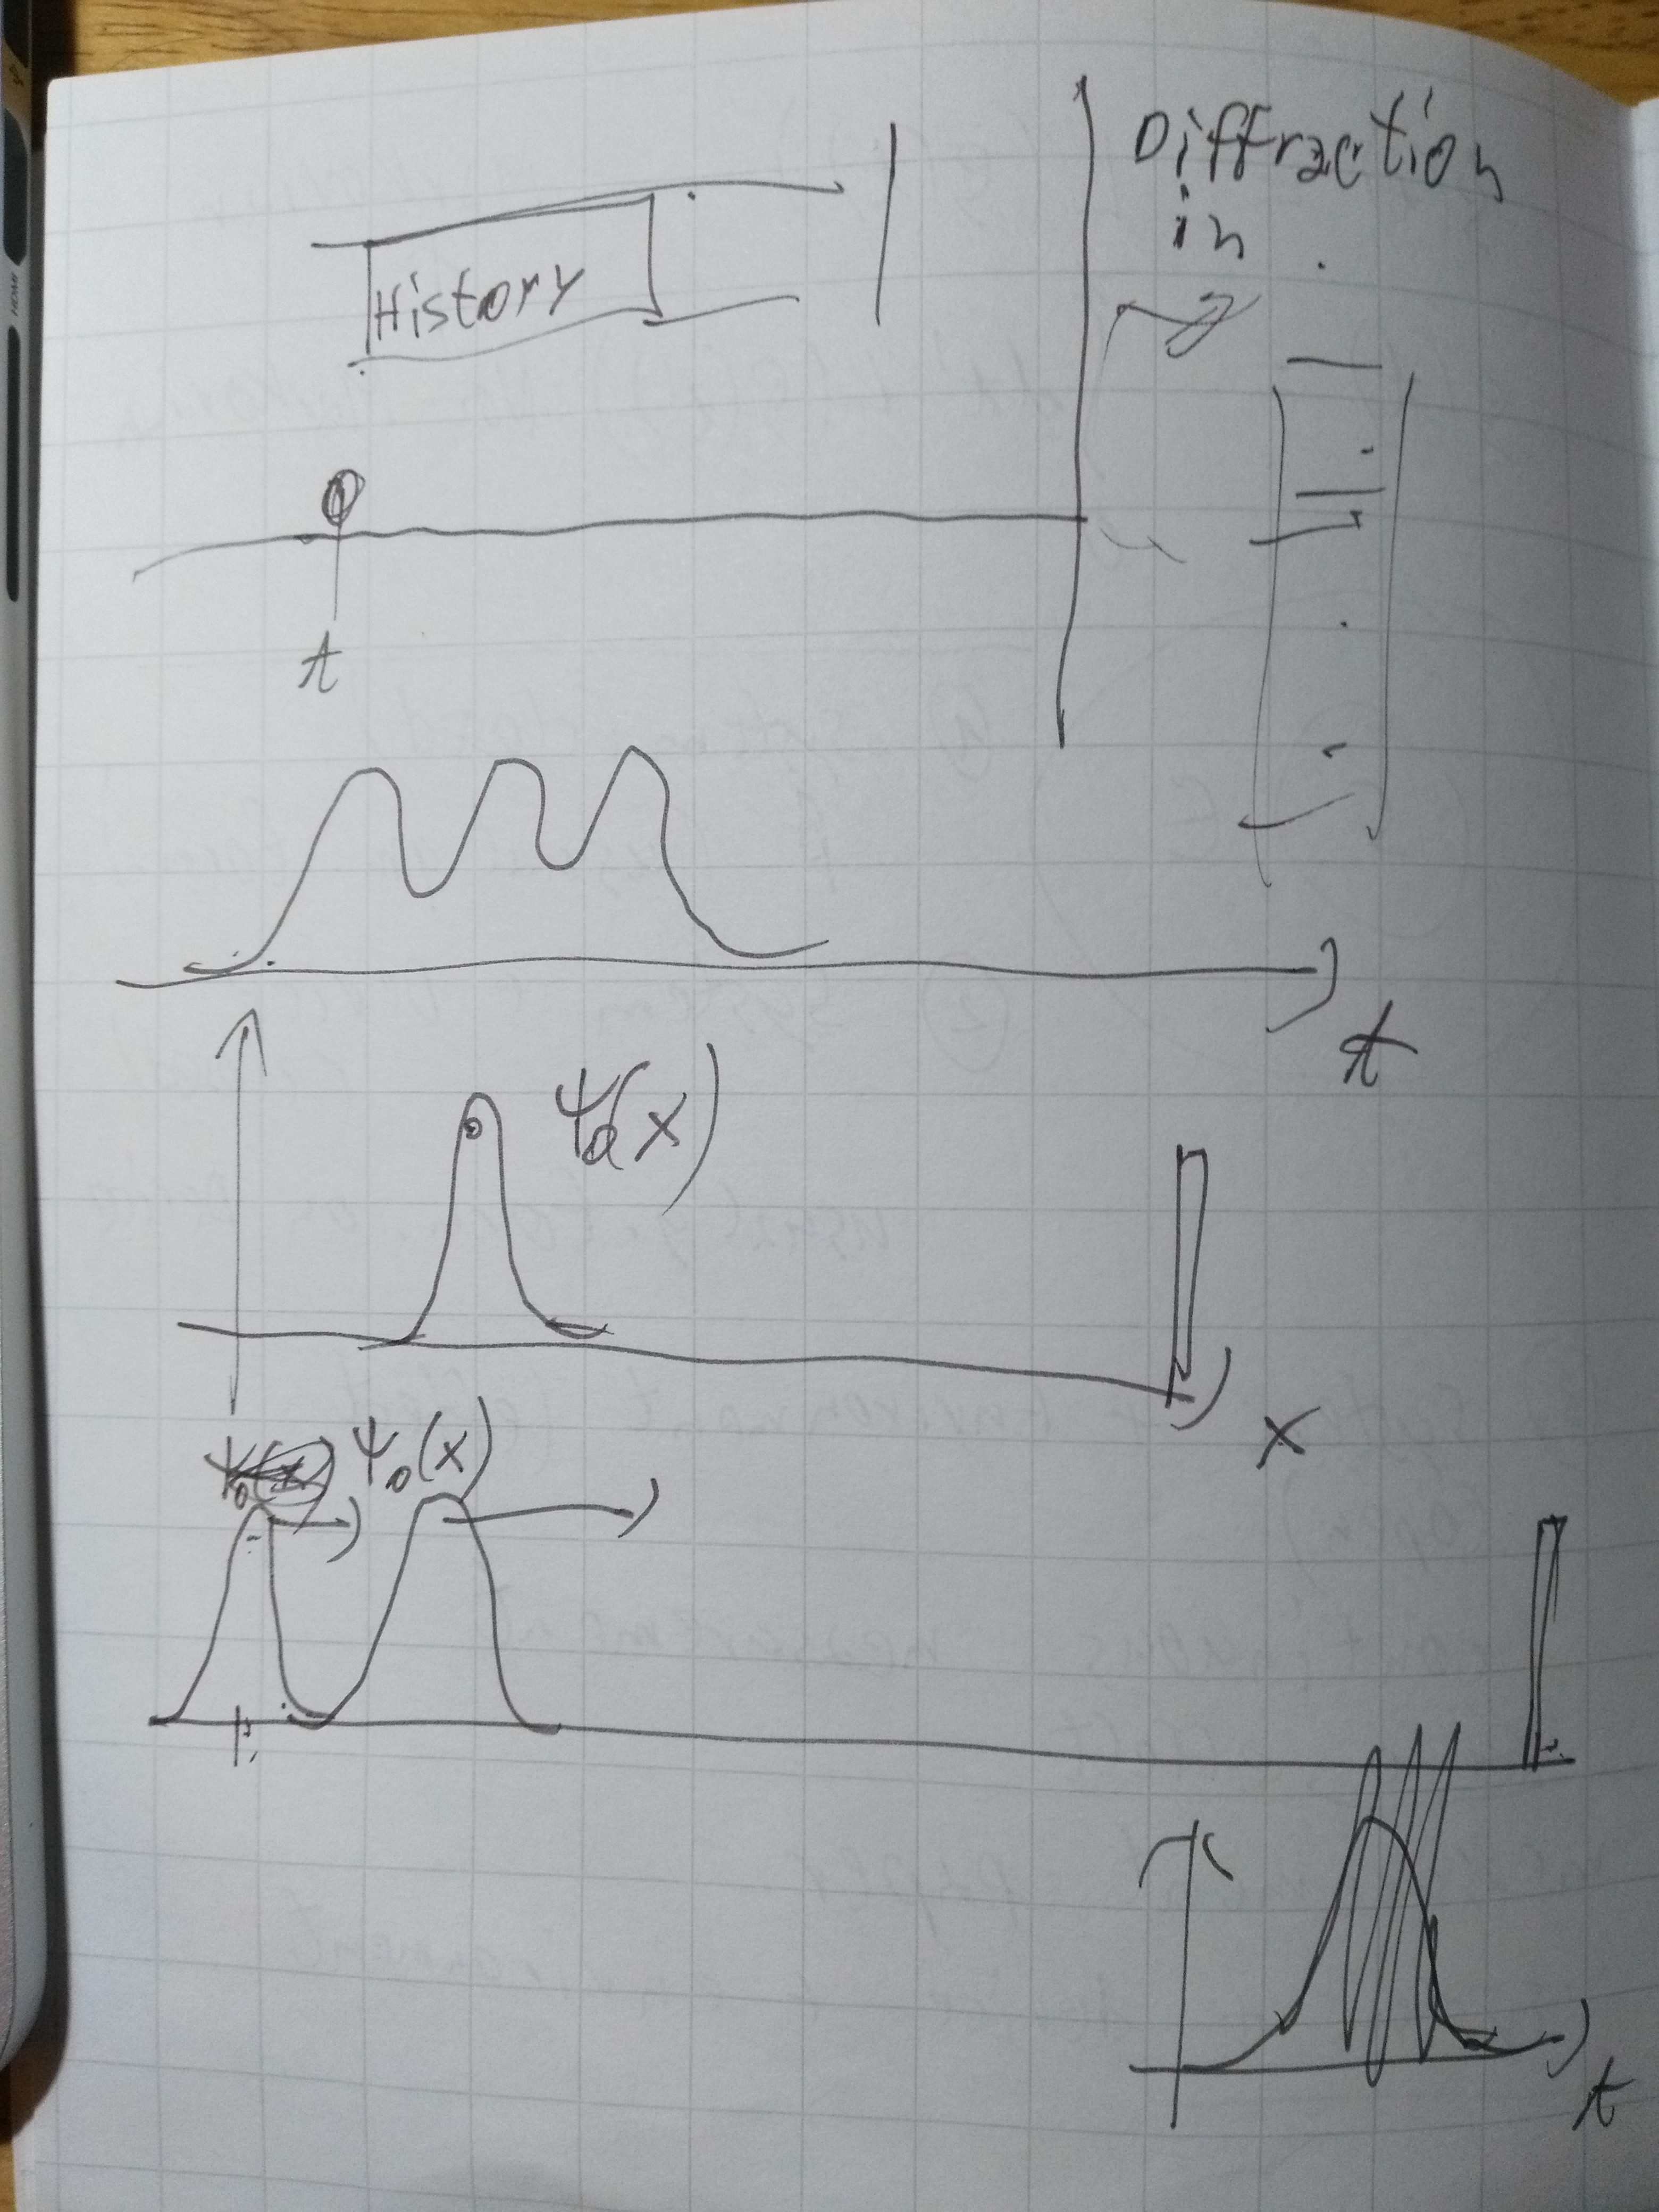
\includegraphics[width=\linewidth]{img/diffraction.jpg}

\section{pw}

Lloyd recent on entropic uncertainty (for time\dots).
From state vectors to density matrices and/or mixed states: Von Neumann entroy (wikipedia).
Subadditivity. 

\section{Misc}

\subsection{Quantum computing, IBM, decomposition, Trotter-SUzuki, Sine-cosine, qubiter dir}

Previous section(s) read(s):
\begin{quote}
  A benefit of finite-dimensional systems is the potential implementation on a finite array of
  qubits in a quantum computer.
\end{quote}
Make a ref from there to here, and talk about qubiter and stuff.

Also, \cite{Moreva:illustration} has FIG.1 gate array repr\dots

\subsection{Quantum Blockchain and Entanglement in Time}

\url{https://spectrum.ieee.org/tech-talk/computing/networks/quantum-blockchains-could-act-like-time-machines}
\url{https://arxiv.org/abs/1804.05979}


\subsection{Misc}

Extra: \cite{TimeAnyons}.

TQM Book: time of residence: applicable to qubits, therefore Moreva experiment.

\url{https://arxiv.org/abs/1708.04302} majorization, thermo.


\subsection{and dwell time}

\cite[\S 5]{TQM2}, \cite{YearsleyHalliwell_Clocks}.

\subsection{In relation with the \term{time of residence}}

Here we compare \cite{Moreva:synthetic, Moreva:illustration}
(a Page and Wootters problem)
with the ``standard'' \term{time of residence}
treated in \cite[\S 5.5.2]{TQM2},
the only usable concept since there is no notion of position
for a qubit.

\subsection{Comparison with (Kijowski/Aharonov-Bohm) time of arrival}

Time of arrival is derived for non-relativistic \parencite{Delgado_TOA, Delgado_TOA2}
and relativisitic \parencite{Leon_TOA_R}
particle.

Kijowski: \cite{Kijowski_Time, Kijowski_Comment}.

\subsection{In relation to Leggett-Garg inequalities}
(Also mentioned in \cite{Moreva_position}).

Ref \cite{LeggettGarg+PageWootters}.

But also Lloyd: \url{https://arxiv.org/abs/1608.05672},
\emph{Decoherent histories approach to the cosmological measure problem}.
Lindbladt, Markov, Open Systems.

Halliwell, \url{https://arxiv.org/abs/1604.01659}. Ancilla, decay (spontaneous emission?).

A phylosophical object to decoherent histories / Everett (Everett mentioned in Marletto/ref)
is at
\url{https://arxiv.org/abs/1603.04845}.



\subsection{On ``taking time seriously'' (time is real) and why it can still be real in Page and Wootters}

No, Smolin
(\term{Time Reborn}, \term{The Singular Universe and the Reality of Time})
pushes this too far, even Special Relativity's time is too ``virtual'' for him.
Similarly, the philosopher Tim Maudlin

\url{https://www.quantamagazine.org/a-defense-of-the-reality-of-time-20170516/}

Here instead we just argue that the clock can actually be really time, not any observable.
We use notation $T$ as in time instead of $C$ as in clock etc.

In this sense, the Moreva experiment is a quantum analogue simulation.


\section{Time crystals}

References: \cite{crystal2,crystal3,crystal2012}.


\section{Irrev}

\cite{Maccone:Pauli} \S IV.  UNBOUNDED-ENERGY CLOCKS?

\subsection{Use open quantum systems theory in ``Decoherence and measurement'' chapter}
Schmidt decompositions, spatial and temporal states in
$\hilb{H}_T$ and $\hilb{H}_S$
are described as density operators
(mixed states). What if there isn't a ``perfect entanglment'' between space and time.

Use the Von Neumann entropy (or other methods) to quantify entanglement?

When the entanglement is perfect, the notion of time evolution emerges, just
like between two dimensions n space, it may or may not ``emerge'' that
$y$ ``depends'' upon $y$ for a given distribution of positions.

\section{Entanglement and decoherence (Arrow of time)}
See also \cite{EntanglementVsDecoherence}.

Decoherence is an irreversible process, it also happens in measurement.

According to Marletto and Vedral, arrow of time is increase in Entanglement
between the clock and the rest.

So, there seems to be a contradiction: is entanglement ``decreasing''
(i.e. destroyed by decoherence) with time
or increasing?

We can avoid the contradiction saying that
entanglement between two finite systems is
destroyed while the entanglement of each of them with the universe
is increasing.

\subsection{``Harmonic clocks''}

Use the harmonic oscillator in \cite{HarmonicClocks}
as a PaW clock for the same packet that is measured in
Ruschhaupt's detector model.

Therein, fading wave function: is minus derivative an event?
L4 normalized?


\subsection{Misc}

Idea: use section B ``Measurement'' of \cite{Lloyd:Time}: detector as (binary) measument device.

``Philospher'': \url{https://arxiv.org/abs/1704.07236}.

Time of arrival and clocks: again, \cite{YearsleyHalliwell_Clocks}.
Which maybe suggests we should not wory too much of $H\ket{\Psi} = 0$. 

We don't. 

BUT please note \cite{YearsleyHalliwell_Clocks} uses a clock that is
\emph{coupled} with the system, while in PaW they are ``only'' entangled.
So their calculation may be unnecessarily complicated.
Maybe the weakjly coupling case can be used?

Other systems of interest: decays. Prvanovic new.

Reference \cite{ConnesRovelliThermo}.

Relate with John Goold's works? The ancilla as a clock? --- Topical Review

Markovianity, histories.

Lloyd on arXiv: from clock to cloners; erasing; scrambling (as in Goold).

Lloyd on decoherent histories (Gellman, Hartle?).

Dechoerence / irreversibility / measurement.

Vedral / Lloyd. Discord.

Measuring entanglement: Quantification of Concurrence via Weak Measurement: 1611.00149.

Marletto/Vedral on Arrow of time. Arrow of time as increasing entanglement.

Arrow of time: 

\url{https://www.wired.com/2014/04/quantum-theory-flow-time/}

\url{https://en.wikipedia.org/wiki/Loschmidt%27s_paradox}

\url{https://www.quantamagazine.org/20160119-time-entanglement/}

\url{https://arxiv.org/pdf/1702.07706.pdf} \textit{The second law of thermodynamics at the microscopic scale}
Thibaut Josset,
Aix Marseille Univ. (David).

Maxwell's demon: https://arxiv.org/pdf/1702.05161.pdf

\subsection{and paths}

Both \cite{YearsleyHalliwell_Clocks} and \cite{Gambini_PW}
reason in terms of paths and actions, maybe Feynmann stuff
in following chapter... and maybe conistent historiesapproach can help
towards linking PaW and ToA?

Also \url{http://quantum.phys.cmu.edu/CHS/CHS_transp.pdf}.

\subsection{Decays?}

We might want to look at exponential decay from \url{https://arxiv.org/abs/1704.07236},
then compare with exponential decay with P and W using Lloyd Giovannetti and Maccone (ref).

\subsubsection{Purification}

See https://arxiv.org/pdf/quant-ph/0512125.pdf, P-W time as a purifying ancilla
of the (Kijowski?) time.

\section{Misc/Multi/Extras/Outlook}

\url{https://arxiv.org/abs/1703.05876}
--- \emph{comment}: time measured and stored here
may be all classical information
so this paper may or may not be relevant for the topic.

But
``prototypes of clocks based on quantum principles,
such as entanglement and squeezing''
may make this interesting again, see reference therein.
They also cite Lloyd, Giovannetti and Maccone,
but a paper quite older than \cite{Lloyd:Time}.

\url{https://arxiv.org/abs/1603.02522}
\emph{Decoherence by spontaneous emission: a single-atom analog of superradiance}.
Decoherent histories, non-markovianity, open quantum systems.

\url{https://arxiv.org/abs/1007.2615} Time travel / Quantum CTC.

Carmichael et al. \cite{CarmichaelOQS2017} (Andreas's reading)
(non-markovianity).

Non-markovian, quantum-to-classical, open systems, David,
\url{https://arxiv.org/pdf/1703.09428.pdf}.

In his works, Zurek mentions:
DeWitt, Everett, gell_Mann, hartl, Many Worlds, consistent/decoherent histories:
idea: Lagrangian over a history? Principle of least action?

Zurek: ``Reduction of the Wavepacket: How Long Does it Take?'' (arxiv),
``quantum''' time? \cite{Zurek_Einselect} also mentions
``decoherence timescale''.

Von Neumann/Shannon entropy in measurement? Mention information problems
in quantum cosmology (where a quantum time is necessary)? Etc. etc.

\section{for Relativistic treatment}

\cite{RealisticClocks}.

\cite{HarmonicClocks} concludes ``Classical clock can be described by an Hamiltonian linear in momentum''\dots
like in relativity?

\cite{Lloyd:Time} does not only deal with improper eigenstates in $\hilb{H}_T$
(full evolutions?)
but also normalized ones (in $\hilb{H}_T$! \emph{``Events''}?)

A Page and Wootters time of arrival is mentioned in \cite{Gambini_PW}.

\subsection{Time-of-arrival for a Klein-Gordon free particle}

See \cite{Galapon_KG}.

\subsection{Feynmann path stuff}

Sokolovski 1703.01966, Feynmann paths...\subsection{(dis)entanglement under gravity, decoherence, event formalism}

1703.08036 An experiment to test decoherence under gravity aka entangled photons undergoing different paths and how their entanglement is affected.
``Space QUEST mission proposal: Experimentally testing decoherence due to gravity''.

Are they getting entangled with the environment instead? (Merletto and Vedral).

The theoretical paper behind the space experiment: \url{https://arxiv.org/pdf/1406.3677.pdf}. Interestingly, it mentions 
\emph{event formalism}, and we thought about that: is an event something
representable as a proper vector in $\mathcal{L}^2(\mathbb{R}^4)$ --- where one of the dimensions is time?
Deepen the event formalism if it's quantum.

Resume ``Quantum Statistical Gravity''? \url{https://arxiv.org/abs/1602.05707}.

``Fundamental decoherence from quantum gravity: a pedagogical review''
\url{https://arxiv.org/abs/gr-qc/0603090} ---
``fundamental loss of unitarity
that appears in quantum mechanics
due to the use of a physical apparatus to measure time''.

Closed timelike curves are also the subject of a paper by Lloyd (cite!).

``Deutsch argued that
the usual paradoxes associated with such solutions of general
relativity can be resolved by quantum mechanics''  in the reference above. But in the even formalism
\emph{spacetime is still a classical background!}. Event operators a parametrized by $t$\dots

\subsection{Prvanovic and P\&W}
In \cite{Prvanovic}, essentially the clock observable is the Hamiltonian.
The two example clocks are an harmonic oscillator and a free particle.
The harmonic oscillator features discrete time. Generally a time which is
{bounded from below}
is consistent with the Big Bang...

Prvanovic uses ``relativisitc'' constants...

BTW, please note a time bounded from below WOULD NOT be sufficient to overcome the Pauli objection alone.





\appendix
\chapter{Commutator properties}
\section{Power}
\begin{lemma}\label{CommProp}
If the commutator $[T, H]$ commutes with $T$ i.e.
$$[T, H]T~=~T[T, H]\,,$$ then the following holds:
\begin{equation}\label{eq:tkh}
[T^k, H] = kT^{k-1}[T, H]\,.
\end{equation}
\end{lemma}
This is particularly true when $[T, H]$ is a \emph{number} as in \eqref{THcommutator} where
$T$ and $H$ are the time and energy operator respectively.
\begin{proof}
First of all, the \eqref{eq:tkh} is trivially valid for $k = 1$.

For an arbitrary positive integer $k$ there has:
\begin{dmath}\label{tkhrecur}
[T^k, H] = T^{k-1}TH - HT^{k-1}T = T^{k-1}TH - T^{k-1}HT + T^{k-1}HT - HT^{k-1}T \\
    = T^{k-1}[T, H] + [T^{k-1}, H]T
\end{dmath}
Now, iterating the result in \eqref{tkhrecur},
\begin{dmath}\label{tkhrecurplus}
[T^k, H] = T^{k-1}[T, H] + [T^{k-1}, H]T
= T^{k-1}[T, H] + (T^{k-2}[T, H] + [T^{k-2}, H]T)T
= T^{k-1}[T, H] +  T^{k-1}[T, H] + [T^{k-2}, H]T^2
= 2T^{k-1}[T, H] + [T^{k-2}, H]T^2
= \hdots
= nT^{k-1}[T, H] + [T^{k-n}, H]T^n = \hdots
\end{dmath}
where the commutativity hypothesis $[T, H]T = T[T, H]$ has been used to obtain $T^{k-2}[T, H]T = T^{k-1}[T, H]$.

Now, \eqref{tkhrecurplus} can be continued until it reaches $n=k$ when the term
$[T^{k-n}, H]T^n$ vanishes and a result of $kT^{k-1}[T, H]$ follows.
\end{proof}

\chapter{Density operators, projectors and measurement}
\section{Projectors}

We shall assume, unless otherwise stated, that all vectors are
normalized to unity.

For a given observable represented by an operator $A$ with a
\emph{discrete, non degenerate spectrum}, the probability of the
outcome $a$ of a
measurement on a system in the pure state $\ket{\psi}$ is given by
$$
\pi_{a} = \norm{\braket{a}{\psi}}^2
        = \bra{\psi}\ket{a}\bra{a}\ket{\psi}
        = \mel{\psi}{P_{a}}{\psi}
$$
where $P_{a} = \ketbra{a}$ appears as the \term{projector} on the
one-dimensional eigenspace of  $a$.

If $a$ is degenerate, and $j = 1, \dots, J$ its degeneracy index,
such probability shall sum over it:
$$
\pi_{a} = \sum_{j=1}^{J}\norm{\braket{aj}{\psi}}^2
        = \sum_{j=1}^{J}\bra{\psi}\ket{aj}\bra{aj}\ket{\psi}
        = \mel{\psi}{P_{a}}{\psi}
$$
where $P_{a} = \sum_{j=1}^{J}\ketbra{aj}$
still is the projector on the
($J$-dimensional) eigenspace of $a$.

Generally, the probability that the outcome of a measuremen falls in
the set of eigenvalues $\sigma = \{a_{1}, \dots, a_{S}\}$ is
\begin{equation}\label{eq:pi_sigma}
\pi_{\sigma}  = \sum_{s=1}^{S}\sum_{j=1}^{J_{s}}\norm{\braket{sj}{\psi}}^2
              = \sum_{s=1}^{S}\sum_{j=1}^{J_{s}}\bra{\psi}\ket{sj}\bra{sj}\ket{\psi}
              = \mel{\psi}{P_{\sigma}}{\psi}
              ,
\end{equation}
where $P_{\sigma} = \sum_{s=1}^{S}\sum_{j=1}^{J_{s}}\ketbra{sj}$
is once again a projector --- on the ``generalized eigenspace'' spanned by all
eigenvectors $\{\ket{sj}\}$ above.

\section[Measure]{Measure\footnote{Not to be confused with \emph{measurement}.}}

\begin{remark}\label{measure_properties}
  Being $\pi_{\sigma}$ the \emph{probability} of the outcome of a measurement to
  fall in a given set $\sigma$, it has to be:
  \begin{enumerate}
    \item \label{measure_properties:first} $0$ on the empty set
    \item non negative
    \item \label{measure_properties:last} \term{additive} on disjoint sets
    \item equal to $1$ if $\sigma$ includes the whole spectrum of $A$.
  \end{enumerate}
\end{remark}

\begin{remark}
  Properties \ref{measure_properties:first}\dots\ref{measure_properties:last}
  are the defining properties of a \term{measure} \parencite{EncMath_Measure}.
\end{remark}

The probability $\pi_{\sigma}$ in \eqref{eq:pi_sigma} is linear with respect to the projector
$P_{\sigma}$ hence it's not difficult to derive that the same properties in
\autoref{measure_properties} applies to $P_{\sigma}$, \emph{in the operator sense}.
In fact, the map $\sigma \subseteq \mathbb{R} \rightarrow P_{\sigma}$
implicitly defined in~\eqref{eq:pi_sigma} is a \term{projector-valued measure}.

The result is generalized,
in such a way to include both discrete and continous spectra,
by the following \cite{VonNeumann, Ballentine}
\begin{theorem}[spectral resolution]
  If $A$ is a self-adjoint operator,
  there is a unique projector-valued measure $E$
  defined on the Borel sets of $\mathbb{R}$
  such that
  \footnote{
    In \eqref{eq:spectral}, $a$ is a real number (not a set),
    but it's intended $E$ to be evaluated
    on the~\emph{interval}~from $-\infty$ to $a$.
  }
  \begin{equation}\label{eq:spectral}
    A=\int_{-\infty}^{\infty}a\, dE(a)
  \end{equation}
  and satisfying:
  \begin{align*}
    E(\mathbb{R})       & =\mathbf{1},\\
    E(B_{1}\cap B_{2}) & =E(B_{1})E(B_{2})\,.
  \end{align*}
\end{theorem}

In terms of this theorem, the projector in \eqref{eq:pi_sigma} is
\begin{equation}\label{eq:P_sigma_spectral}
  P_{\sigma} = E(\sigma) = \int_{a\in\sigma}dE(a)
\end{equation}
and $dE(a)$ is
---informally speaking---
infinitesimal if $a$ belongs to the continous spectrum,
finite if $a$ is a discrete eigenvalue
and zero otherwise.

\section{Density operator}\label{app:density}

The above results apply to \term{pure states}.
More generally, a quantum state (either pure or \term{mixed}),
is described by a \term{density} (or \term{state}) operator $\rho$.
It's a well known result (see, for example, \cite{open_systems})
that the expectation value of an observable represented by the operator $A$
is given in this description by
\begin{equation}\label{eq:expvalA_rho}
  \expval{A} = \tr(A\rho)\,.
\end{equation}

The \eqref{eq:expvalA_rho} is valid for any hermitean operator $A$,
hence we can replace it with the projector $P_{\sigma}$,
associated to the set of eigenvalues $\sigma$
according to \eqref{eq:pi_sigma} and \eqref{eq:P_sigma_spectral},
which is of particular interest
because its mean value equates the probability that the outcome of a measurement
falls in a given subset of the spectrum of a given observable.
Hence we can derive:

\begin{proposition}\label{probability_rho}
  The probability $\pi_{\sigma}$
  that the outcome of a measurement of the observable $A$
  on the system described by the state operator $\rho$
  falls in the set $\sigma$
  is given by:
  \begin{equation}\label{eq:probability_rho}
    \pi_{\sigma} = \expval{P_{\sigma}} = \tr(P_{\sigma}\rho)
  \end{equation}
  with $P_{\sigma}$ defined as in \eqref{eq:pi_sigma}
  or, more generally, in \eqref{eq:P_sigma_spectral}.
\end{proposition}

\subsection{Properties of the density operator}
\subsubsection{Additivity}
The general expression for a density operator $\rho$ is
$$
  \rho = \sum_{k}p_{k}\ketbra{\psi_{k}}
$$
with $p_{k}$ non negative and $\sum_{k}p_{k} = 1$.

The condition is not restrictive to prevent proving the following
\begin{proposition}
  Let $A$ be an hermitean operator such that
  $$
    \tr(A\rho) = 0 
  $$
  \emph{for any density operator} $\rho$.

  It follows that $A = 0$.

  \begin{proof}
    We can choose,
    as basis to explicit the expresion of the trace,
    a complete set of eigenvectors $\{\ket{m}\}$ of $A$ and,
    for each positive integer $n$,
    a particular density operator $\rho = \ketbra{n}$,
    corresponding to a (pure) eigenstate of $A$.

    With this particular choice,
    for each $n$,
    $$
      A\rho = \mel{n}{A}{n}\ketbra{n}\,.
    $$
    It then follows:
    $$
      0 = \tr(A\rho) = \sum_{m}\mel{m}{ ( \mel{n}{A}{n}\ketbra{n} ) }{m}
        = \sum_{m} \mel{n}{A}{n} \braket{m}{n} \braket{n}{m}
        = \mel{n}{A}{n}\,,
    $$
    hence the generic diagonal element of the (diagonal) matrix of $A$ is null,
    and so is consequently the operator $A$ itself.
  \end{proof}
\end{proposition}

\begin{corollary}
If $\tr(A\rho) + \tr(B\rho) = \tr(C\rho)$ for any density operator $\rho$,
then $A + B = C$.
\end{corollary}


\bibliographystyle{IEEEtran}
\bibliography{biblio}

\end{document}